% !TEX TS-program = XeLaTeX
% use the following command:
% all document files must be coded in UTF-8
\documentclass[english]{textolivre}
% build HTML with: make4ht -e build.lua -c textolivre.cfg -x -u article "fn-in,svg,pic-align"

\journalname{Texto Livre}
\thevolume{19}
%\thenumber{1} % old template
\theyear{2026}
\receiveddate{\DTMdisplaydate{2026}{2}{5}{-1}} % YYYY MM DD
\accepteddate{\DTMdisplaydate{2026}{3}{6}{-1}}
\publisheddate{\DTMdisplaydate{2026}{7}{17}{-1}}
\corrauthor{Sigrid Ørevik}
\articledoi{10.1590/1983-3652.2026.64269}
%\articleid{NNNN} % if the article ID is not the last 5 numbers of its DOI, provide it using \articleid{} commmand 
% list of available sesscions in the journal: articles, dossier, reports, essays, reviews, interviews, editorial
\articlesessionname{dossier}
\runningauthor{Diamantopoulou and Ørevik} 
%\editorname{Leonardo Araújo} % old template
\sectioneditorname{Fei Victor Lim~\orcid{0000-0003-3046-1011}}
\layouteditorname{Leonardo Araujo~\orcid{0000-0003-3884-2177}}

\title{A multimodal social semiotic rethinking of agency in AI-assisted designs for language learning and assessment: Examples from Duolingo}
\othertitle{Repensando a agência sob uma perspectiva sociossemiótica multimodal em designs assistidos por IA para aprendizagem e avaliação de línguas: exemplos do Duolingo}
% if there is a third language title, add here:
%\othertitle{Artikelvorlage zur Einreichung beim Texto Livre Journal}

\author[1]{Sophia Diamantopoulou~\orcid{0000-0001-8564-8743}\thanks{Email: \href{mailto:sophia.diamantopoulou@ucl.ac.uk}{sophia.diamantopoulou@ucl.ac.uk}}}
\author[2]{Sigrid Ørevik~\orcid{0000-0002-0812-4572}\thanks{Email: \href{mailto:sigrid.orevik@uib.no}{sigrid.orevik@uib.no}}}
\affil[1]{University College London, Institute of Education, London, United Kingdom.}
\affil[2]{University of Bergen, Department of Foreign Languages, Bergen, Norway.}

\addbibresource{article.bib}
% use biber instead of bibtex
% $ biber article

% used to create dummy text for the template file
\definecolor{dark-gray}{gray}{0.35} % color used to display dummy texts
\usepackage{lipsum}
\SetLipsumParListSurrounders{\colorlet{oldcolor}{.}\color{dark-gray}}{\color{oldcolor}}

% used here only to provide the XeLaTeX and BibTeX logos
\usepackage{hologo}

% if you use multirows in a table, include the multirow package
\usepackage{multirow}

% provides sidewaysfigure environment
\usepackage{rotating}

% CUSTOM EPIGRAPH - BEGIN 
%%% https://tex.stackexchange.com/questions/193178/specific-epigraph-style
\usepackage{epigraph}
\renewcommand\textflush{flushright}
\makeatletter
\newlength\epitextskip
\pretocmd{\@epitext}{\em}{}{}
\apptocmd{\@epitext}{\em}{}{}
\patchcmd{\epigraph}{\@epitext{#1}\\}{\@epitext{#1}\\[\epitextskip]}{}{}
\makeatother
\setlength\epigraphrule{0pt}
\setlength\epitextskip{0.5ex}
\setlength\epigraphwidth{.7\textwidth}
% CUSTOM EPIGRAPH - END

% to use IPA symbols in unicode add
%\usepackage{fontspec}
%\newfontfamily\ipafont{CMU Serif}
%\newcommand{\ipa}[1]{{\ipafont #1}}
% and in the text you may use the \ipa{...} command passing the symbols in unicode

% LANGUAGE - BEGIN
% ARABIC
% for languages that use special fonts, you must provide the typeface that will be used
% \setotherlanguage{arabic}
% \newfontfamily\arabicfont[Script=Arabic]{Amiri}
% \newfontfamily\arabicfontsf[Script=Arabic]{Amiri}
% \newfontfamily\arabicfonttt[Script=Arabic]{Amiri}
%
% in the article, to add arabic text use: \textlang{arabic}{ ... }
%
% RUSSIAN
% for russian text we also need to define fonts with support for Cyrillic script
% \usepackage{fontspec}
% \setotherlanguage{russian}
% \newfontfamily\cyrillicfont{Times New Roman}
% \newfontfamily\cyrillicfontsf{Times New Roman}[Script=Cyrillic]
% \newfontfamily\cyrillicfonttt{Times New Roman}[Script=Cyrillic]
%
% in the text use \begin{russian} ... \end{russian}
% LANGUAGE - END

% EMOJIS - BEGIN
% to use emoticons in your manuscript
% https://stackoverflow.com/questions/190145/how-to-insert-emoticons-in-latex/57076064
% using font Symbola, which has full support
% the font may be downloaded at:
% https://dn-works.com/ufas/
% add to preamble:
% \newfontfamily\Symbola{Symbola}
% in the text use:
% {\Symbola }
% EMOJIS - END

% LABEL REFERENCE TO DESCRIPTIVE LIST - BEGIN
% reference itens in a descriptive list using their labels instead of numbers
% insert the code below in the preambule:
%\makeatletter
%\let\orgdescriptionlabel\descriptionlabel
%\renewcommand*{\descriptionlabel}[1]{%
%  \let\orglabel\label
%  \let\label\@gobble
%  \phantomsection
%  \edef\@currentlabel{#1\unskip}%
%  \let\label\orglabel
%  \orgdescriptionlabel{#1}%
%}
%\makeatother
%
% in your document, use as illustraded here:
%\begin{description}
%  \item[first\label{itm1}] this is only an example;
%  % ...  add more items
%\end{description}
% LABEL REFERENCE TO DESCRIPTIVE LIST - END


% add line numbers for submission
%\usepackage{lineno}
%\linenumbers

\begin{document}
\maketitle

\begin{polyabstract}
\begin{abstract}
This article addresses issues of design and agency, focusing on Artificial Intelligence (AI)-generated tools for speaking practice and assessment in the field of English language learning. It uses examples from the educational technology company Duolingo as agentive designs for enabling and assessing learning. Drawing on multimodal social semiotics (MMSS) as a theoretical and methodological lens, the article analyses selected screenshots from the Duolingo examples as multimodal texts-in-action, showcasing how these AI-assisted learning designs make visible the agency of the designer and the role of AI, and how the design facilitates the user’s agency. In these designs, AI is described as enacting a form of devolved agency, given that it interacts with the user as a proxy for the human designers who shape the affordances of the AI-assisted learning design. Among the implications of the study is an identified need to make more visible the limitations and potential of MMSS theory to account for the role of AI in contexts of learning and communication.

\keywords{Agency \sep Designs for learning \sep Multimodal social semiotics \sep English language learning \sep Artificial intelligence}
\end{abstract}

\begin{portuguese}
\begin{abstract}
Este artigo aborda questões de design e agência, com foco em ferramentas geradas por Inteligência Artificial (IA) para a prática oral e sua avaliação no campo da aprendizagem de língua inglesa. Utilizam-se exemplos da empresa de tecnologia educacional Duolingo como designs agentivos para facilitar e avaliar a aprendizagem. Tendo como base teórica e metodológica a semiótica social multimodal (multimodal social semiotics – MMSS), o artigo analisa capturas de tela selecionadas dos exemplos do Duolingo como textos multimodais em ação, mostrando como esses designs de aprendizagem assistidos por IA tornam visível a agência do designer e o papel da IA, e como o design facilita a agência do usuário. Nesses designs, a IA é descrita como desempenhando uma forma de agência delegada, uma vez que interage com o usuário como uma representante dos designers humanos, os quais moldam as capacidades (\textit{affordances}) do design de aprendizagem assistido por IA. Entre as implicações do estudo, identifica-se a necessidade de tornar mais visíveis as limitações e o potencial da teoria MMSS para explicar o papel da IA em contextos de aprendizagem e comunicação.

\keywords{Agência \sep Designs para aprendizagem \sep Semiótica social multimodal \sep Aprendizagem de língua inglesa \sep Inteligência artificial}
\end{abstract}
\end{portuguese}
% if there is another abstract, insert it here using the same scheme
\end{polyabstract}

\section{Introduction}\label{sec-intro}
\subsection{Overview and argument}
This article raises questions of agency in the context of new developments in designing for language learning and assessment with Artificial Intelligence (AI). As the design of tools for learning in educational contexts increasingly involves AI, relevant scholarly work is also engaging with the affordances of new AI technologies, issues of agency and the way AI shapes learning, teaching and assessment in this new landscape of communicative language learning with technology \cite{cope2021education,karatza2024multimodal,lim2025editorial}. Building on a conference paper \cite{vondavier2025designing} which researched agency in designs for language learning using examples from Duolingo – an educational technology company known for its development of a language learning app and the Duolingo English Test (DET) – this article focuses on how agency is enacted and facilitated in such designs.

Aiming to showcase distinct and diverse approaches to integrating AI in language learning and assessment, we have selected examples from three AI-powered features of the Duolingo app – ‘Video Call with Lily’, ‘Role Play’ and ‘Explain My Answer’ – along with excerpts from the Interactive Speaking component of the Duolingo English Test. The selected AI-powered features are designed for independent and informal conversation practice with a chatbot, while the Interactive Speaking component of DET is part of a high-stakes online test for a language qualification, where control and regulation are expected.

Drawing on multimodal social semiotic (MMSS) theorisations of design, learning and agency \cite{bezemer2016multimodality,kress2010multimodality,selander2017design,diamantopoulou2024design}, we explore their relevance for making sense of the role of AI and humans in these designs. A starting point in our research is the MMSS position that every design for learning realises the designers’ agency, rhetoric and interest \cite{bezemer2016multimodality}. With this in mind, we ask how the selected Duolingo AI-assisted multimodal designs make visible the agency of the designers and the role of AI, as well as how the user’s agency is enabled.

Through our analysis, we argue that AI has a form of agency, namely, the devolved agency of multiple human agents and voices shaping the affordances of the AI, and acts as a proxy for human agency. This devolved agency is performed and simulated. In other words, we argue that a performative, devolved, simulated agency can be evident in AI-assisted designs for language learning, and is pertinent to examples used here. However, we acknowledge that studying other instances involving different AI-powered language learning resources may require a rethinking of agency and design in the light of a broader range of theories.

In the following sections, we locate this article within the broader scholarly work on AI, agency and designs for learning in educational contexts, within and beyond multimodality. We then present our theoretical positioning within MMSS and propose an expanded theoretical framework for understanding agency in AI-assisted designs for language learning and assessment. This is followed by contextual information about the role of AI in the selected Duolingo examples, forming a backdrop to the subsequent MMSS-driven analysis.

\section{Literature Review}\label{sec-normas}
Focusing on agency in the AI-assisted Duolingo designs for learning from the intersecting perspectives of MMSS theory and the field of Multimodality in English Language Learning (MELL) \cite{diamantopoulou2025mell} necessitates an engagement with previous research on AI and agency within MMSS and language learning perspectives. However, we identify few relevant precedents bringing these dimensions together \cite{vondavier2025designing}.

Agency and the nature of AI agency have been discussed in scholarly work from numerous theoretical perspectives and disciplines, including the educational and multimodal research contexts which are the focus here. This work – coming from areas such as sociology, philosophy, ethics, machine learning and information systems, AI engineering, and increasingly from interdisciplinary perspectives – illuminates what AI can do and what humans can do with AI. The focus of this scholarly work on aspects of the synergistic relation between humans and technology is a point of reference in our exploration of the potential of MMSS to attend to AI designs.

The discussion about agency ascribed to objects and extending beyond human capacity is not new. For example, \posscite{gell1998art} anthropological theorisation of ‘object agency’ as the ability of material culture to influence human behaviour and social practices is an important precedent. Within the realm of social theory, scholars aligning with the actor-network theory of \textcite{latour2005reassembling}, such as \textcite{tufekci2015algorithmic,bennett2010vibrant}, argue that there are interactions and relations between humans and non-human actants. For instance, \textcite{tufekci2015algorithmic} assigns active agency to digital technologies in the shaping of social movements. Along similar lines, \textcite{bennett2010vibrant}, in the field of political theory, recognises the agency of non-human entities as interwoven with human agency, in her theorisation of ‘distributive agency’. Her understanding of agency as “a confederation between human and non-human elements” \cite[p. 21]{bennett2010vibrant} is relevant to our rethinking of \posscite{kress2010multimodality} notion of ‘distributed agency’ in the context of AI-assisted designs for learning.

More recent discussions on the potential agency of AI arise along the lines of similar interdisciplinary work positioning non-human agents within networks and assemblages of human and non-human actants. \textcite{burriss2024critical} – additionally taking up a post-humanist literacy approach – attend to the enactment of agency by AI. They see it as part of the sociomaterial process and relations between humans and AI, and not as an inherent capacity of AI which does not have intentionality.

Discussing AI from the information system perspective, \textcite[p. 3]{agerfalk2020artificial} argues that information systems (IS) have agency in the sense that they “can perform social action with only indirect human intervention”. Establishing the premise that decision making is a constituent aspect of agency, \textcite{swanepoel2024agency}, from the fields of philosophy and AI ethics, argue that AI has limited agency. AI can make decisions based on parameters that can be numerically calculated. However, it does not possess the capacity to exercise a will to choose between two equally valued options, something that fundamentally limits the agency that can be ascribed to AI.

Within the domain of multimodality, Cope and Kalantzis were the first to discuss AI agency, drawing from multiliteracies, multimodal grammar and their design theory \cite{cope2022artificial,cope2024a_multimodal}. They advocate that AI cannot exert agency on its own but can extend human agency. According to them, agency is one of the five functions of meaning – along with reference, structure, context, and interest – which can only be delivered by human intelligence that integrates sensory and emotional faculties in interaction with the world. AI can design texts, but it cannot engage in meaning-making in terms of all its functions, as “meaning is more than text” \cite[p. 146]{cope2024a_multimodal}. Gen AI “buries epistemic provenance” \cite[p. 6]{cope2024a_multimodal} and cannot take context into consideration.

Semiotic perspectives on AI – the broader domain within which we operate – have been explored by previous research (e.g., \textcite{matthews2019ai} and also with a special interest in agency (see \textcite{dondero2025aspects}), or human-AI interaction (e.g., \textcite{zappavigna2025emoji}). Specifically, studying agency within the multimodal social semiotic framework, \textcite{tomalin2025multimodal} reframes the theory to account for AI sign-making, given that MMSS limits the attribution of sign-making and agency exclusively to humans. Addressing the relationship between sign-making and motivation, Tomalin envisions a hierarchy of agency, with AI having the potential to be a sign-maker but not a designer. More specifically, \textcite{tomalin2025multimodal} distinguishes between sign designers, as “the humans who determine the design of the sign” – and have intentionality, agency, responsibility and accountability – and the automated or human sign-makers as the entities “creat[ing] the sign” \cite[p. 235]{tomalin2025multimodal}.

This echoes \posscite{kress2010multimodality} distinction between rhetor and designer. For \textcite{tomalin2025multimodal}, there is partial intentionality and agency ascribed to AI, in varying degrees. He claims that “… the intentionality and agency of the (human) sign designers are manifest in the specification of the sign design” and that “designers vicariously motivate the sign ultimately created by the sign-makers” \cite[p. 239-40]{tomalin2025multimodal}. This implies that human designers have remote agency in the sign-making process of AI, resonating with our argument for assigning devolved agency to AI.

Inspired by Bakhtin’s philosophical and literary view of dialogue and dialogic relations, scholars have debated the agency of AI and its potential for dialogic interaction. These scholars come from fields ranging from science education \cite{tang2025dialogic} and discourse studies \cite{duquepereira2025chatbots} to machine-human interaction and digital communication \cite{karimova2025dialogic}. Drawing on the concept of dialogue, Bakhtinian scholars attend to what unfolds in interaction with AI at the level of design and use, with some seeing AI as a dialogue partner and others being sceptical about it.

More specifically, \textcite{tang2025dialogic} identified in students’ chatlogs with Gen AI four prominent dialogic characteristics as evidence of real dialogue: perspective-taking, reasoning, arguing, and creative thinking. While attending to the dialogic characteristics in the AI studied here, we claim that these are evidence of simulated and performed dialogue. AI as an interlocutor is not immersed in social discourses; the social institutional positioning it seemingly endorses is based on numerical values and not the social shaping of its identity. Our view echoes \posscite{duquepereira2025chatbots} position on the simulated nature of conversations with AI. They introduce the term ‘algorithmic monologism’ to account for the fact that although “AI simulat[es] many voices […] they all pass through the same algorithmic filter” \cite[n.p.]{duquepereira2025chatbots}. For them, “what we see is a performance – a dialog simulation produced by an algorithm” \cite[n.p.]{duquepereira2025chatbots}.

Karimova, another Bakhtinian scholar, points to the dimension of dialogic interactions happening at the design level between the designers and AI, observing that “the dialogical nature of relationships between stakeholders involved in many stages of the AI development process seems to be overlooked” and is largely unchartered \cite[p. 3625-6]{karimova2025dialogic}. Although this is not researched in this study, this suggests something fundamental happening at a design level, in our case between the Duolingo designers and AI.

Within the broader educational research, beyond multimodality, including Ed Tech, when scholars focus on AI- or digital technology-assisted learning and agency, they predominantly engage with the learner’s perspectives and outputs, and less with designing for learning with AI, with a significant body of this work focusing on language learning \cite{garzon2025systematic}. When the scholarly attention is on the AI designs and on those designing for learning in AI-assisted environments, the research focus is more on the agency of teachers, their shifting roles as facilitators for learning \cite{purba2025ai}, the role of the AI applications as teaching agents, and the balance between AI scaffolding and learner autonomy. Such work also explores the potential benefits of using AI for learning purposes (e.g., \textcite{dai2025agency}), the impact of AI on learner interaction and human/ AI collaboration (e.g., \textcite{seo2021impact}), or the agency of the learner in relation to AI affordances and scaffolding (e.g., \textcite{abrams2025reflexive,brod2023agency,dai2025agency}). This scholarly work forms another point of reference in our exploration of how the Duolingo designs enable the learners’ agency.

Within the Ed Tech context, \textcite{brod2023agency} elaborate on conceptualisations of the learners’ agency, drawing from the disciplinary perspectives of philosophy, education, and psychology. Arguing for a heightened awareness of agentive relations to technologies, they attend to the multi-dimensionality of agency and the different degrees of agency that can be assigned to learners by teachers and teaching agents, such as AI and digital technologies. This implicit acknowledgement of AI as a teaching agent contributes to the discussion of whether AI has agency.

Multimodal research, across the domains of multiliteracies and social semiotics, has attended to agency with designs for learning in mind, as this study does. Key scholars who opened discussions in this realm include \textcite{cope2022artificial,cope2024a_multimodal,cope2024b_cybersocial}, as well as \textcite{lim2025editorial,jiang2025processgenre}. Cope and Kalantzis – with their interest in the affordances of AI in supporting learning, the relationships between AI and humans in educational contexts and the e-learning ecologies \cite{cope2021education} – enable us to think about the agentive co-design of AI and humans (e.g., \textcite{cope2022artificial,cope2024b_cybersocial}).

In their Learning by Design pedagogic framework, Kalantzis and Cope refer to a “balance of design agency of the writer and the AI in what [they] call a cyber-social learning relationship” \cite[p. 11]{karatza2024multimodal}. In terms of affordances, they claim that AI cannot enact all the ‘epistemic virtues’ involved in education, including critical thinking, the ability to identify meanings “distributed between written text and its contexts” \cite[p. 146]{cope2024a_multimodal}. This kind of distribution differs, though, from the distributed aspect of the agency discussed in our study.

The multimodal semiotic tradition increasingly directs attention to AI and learning, with research on multimodal composition in the digital realm being an entry point. This is reflected, for example, in the special issue of \textit{Computers and Composition} \cite{lim2025editorial}, pointing to the necessity of more research in the direction of multimodal composition with AI. We want to complement this focus on the learner by elaborating on the MMSS theoretical framework as a way to account simultaneously for all three parties involved in designing for learning, namely the human designers, the AI and the learner (user).

\section{Theoretical underpinnings and methods}\label{sec-conduta}
\subsection{Multimodal social semiotics as a key theoretical underpinning}
In this study, we are theoretically positioned within a multimodal social semiotic (MMSS) framework in our attempt to extend the notion of agency. We also operate within Multimodality in English Language Learning (MELL) and aim to contribute to this emerging domain sitting at the intersection of multimodal theory and English as a first or additional language \cite{diamantopoulou2025mell}. Our work relates to the underpinning theoretical principles of MELL, that is, understanding communication as multimodal, endorsing extended notions of literacy, viewing learning as embodied and social, and understanding English as global \cite{diamantopoulou2022multimodality,diamantopoulou2025mell}.

In order to account for the role of AI and for the agency of parties involved in designing for language learning, we draw on the MMSS framework as a theory of communication and learning \cite{bezemer2016multimodality,kress2010multimodality}. We apply the MMSS theoretical and methodological resources to make sense of the Duolingo examples for English language interaction, using screenshots of these multimodal ‘texts-in-action’ \cite{jewitt2021editorial}. We attend to how multimodal resources are orchestrated, as these texts unfold in time, constantly being shaped and reshaped in interaction with a user. In particular, we dwell on the concepts of design and agency. Following \textcite{kress2010multimodality}, we regard design as a coming together of semiotic resources in a multimodal text. “Design is about the organization, mapping and planning of semiotic work through the agentive engagement of the meaning-makers, who assess the aptness of resources, aligning them with their rhetorical intentions” \cite{diamantopoulou2026social}; that is, the rhetoric which the design realises.

Both the notions of multimodal design and sign-making are pertinent for describing and assigning meaning to the examples analysed, as they bring attention to different aspects of the semiotic work that takes place. Designing is understood as the materialisation of rhetoric, institutional conditioning and personal interest, while sign-making is the transformation, orchestration and use of socially made resources.

Endorsing the notion of design prompts the obvious questions: \textit{what is this design for? Who designed it? How has the design come to be the way it is?} In the examples we are studying, we identify three potential designs for learning seemingly in interplay: a) the co-design of the language experts and engineers, entailing, for example, the pedagogic logic, institutional dictates and the AI system guardrails, scripts and rules, and user interface; b) the potential design initiated by AI tools (e.g., models for generating a text and instantiating what the designed system prescribes) when prompted by users; c) the design of the user prompting AI in interaction with a bot, such as the characters used across the features in the Duolingo app or in the DET.

The possibility of different designs for learning emerging in relation to a text-in-action paves the way for enquiring into whose agency is reflected in the design at every given moment. In MMSS the concepts of design and agency are inextricably linked, with both of them referring to human semiotic work. Thus, the MMSS theorisation of agency only takes human entities into account.

In \posscite{kress2010multimodality} theory, agency is central in the semiotic work of individuals as they act within and upon the social world through their meaning-making. “Sign-makers and their agency as social actors are in the foreground” \cite[p. 34]{kress2010multimodality}. Within MMSS and its distinct social agenda, agency can be further understood as the rhetorical positioning of meaning-makers within institutional contexts on the basis of their interests \cite{diamantopoulou2024agency}.

\textcite[p. 134]{bezemer2016multimodality} discuss the role of the shaping agent in the sense of a social agent “[attempting] to shape how others engage with the world”. In the context of education, such agents could be the teachers, or designers of learning resources, who create environments that are apt for learning. Rethinking education in a wider sense, according to \textcite[p. 134]{bezemer2016multimodality}, implies a rethinking also of “the task, the power and the agency of the shaping agent”. The new AI-assisted learning landscape prompts such a rethinking, raising the question of whether AI can be a shaping agent, albeit not a social agent.

The MMSS concept of agency as “distributed between the initial sign-maker and the sign re-maker” \cite[p. 25]{bezemer2016multimodality} is a point of reference and precedent in our theorisation. In previous work, we extended this notion of distribution to account for the agency of institutions. These are understood as discursively shaping and/or prompting the semiotic work of the meaning-makers who exercise their agency co-designing with institutions and their dictates. These dictates/ institutional voices are visible as they are materialised in all designers’ multimodal texts. We showcased that both teachers’ and students’ texts bear traces of institutionally shaped resources that they have transformed as designers, thus evidencing the co-present agency of institutions in these instances of co-design. Consequently, agency is not only distributed between the designer and audience at the interpretation stage, but also at the design stage \cite{diamantopoulou2024design}.

AI-assisted designs, such as the Duolingo ones studied here, have in a way challenged the rules of the game between socially shaped agents, thus raising questions about the kind of distribution of agency at both the design stage and interpretation stages. Establishing whether AI is involved in a kind of distribution of agency is to be researched further.

In this article, as a step towards a broader rethinking of the concept of agency through MMSS – a theory created for human semiotic work – we elaborate further on the need to assign an agentive role to AI to account for the sign-making and designs emerging at the interface with the user. Anchored on previous theoretical elaborations on the implicit and delegated agency of AI \cite{diamantopoulou2024design}, here we further substantiate the argument that a multimodal text-in-action involving AI can be the site of negotiation and co-presence of direct human agencies, as well as the performative, devolved and simulated agency of AI \cite{vondavier2025designing}. Assigning partial agency to AI echoes \posscite{tomalin2025multimodal} thinking. However, as explained above, in our work, we do not distinguish between design and sign-making, as Tomalin does.

\subsection{Methodological approach}\label{sec-fmt-manuscrito}
Multimodal social semiotics “provides conceptual tools that focus on the inter-connectedness between the people’s agency, the technologies in use and the social context of meaning-making […]” \cite[p. 161]{jewitt2016social}. Driven by the theory, we operationalise it, using Kress’s methodological framework and methodological tools, as further elaborated by \textcite{jewitt2016social,diamantopoulou2026social}. Our analysis is driven by the methodological question of how texts, such as AI-assisted or generated apps or teaching resources, come to be the way they are.

Duolingo has been chosen as an example of a commercial educational technology company involving AI in language learning. Apart from designing for informal learning with AI, Duolingo also designs for formal assessment through the Duolingo English Test (DET), which entails the use of AI in a different capacity. The choice of the specific examples analysed here – ‘Video Call with Lily’, ‘Role Play’ and ‘Explain My Answer’, along with the Interactive Speaking component of the DET – has been made based on initial observations regarding the different ways in which AI appears to initiate interaction with the user, raising questions about whose agency is at play across those instances.

A systematic analysis of texts, such as the Duolingo AI-assisted designs, would usually require that researchers frame snapshots from the interaction with users as they unfold in time, attending to the different routes these interactions may take. In this instance, we concentrate on the materiality of selected screenshots from publicly available resources with the aim to showcase how agency is visible in the shaping of a multimodal text. We complement this analysis with observations from our own running of demos and practice tests.

To contextualise our analysis, we present insights from Duolingo research and blogs relating to design aspects of these examples. The aim is to understand how the role of AI in these designs was engineered for purposes of language learning and assessment. Making sense of this entails focusing on the decisions made by the designers in relation to the role of AI in the interaction with the user (e.g., degree of initiative, control, restriction and reactive responses). This enables us to subsequently discuss aspects of the design rationale, including the interests, rhetoric and pedagogical positioning of the designers.

The focus of the MMSS inquiry in the specific screenshots chosen is the identification of the rhetoric and agency of the contributing agents, materialised in the design. Applying the theory, we evidence how the materiality of these designs reflects and makes visible signs of agency, with the assumption being that the multimodality of the designs can be evocative of the designers’ agency, e.g., bearing traces of the designers’ institutional alignment and epistemological positioning.

The process of analysis involves: a) identifying the semiotic resources (modes and modal resources) that work in synergy in the selected screenshots; b) reflecting on the significance of their orchestration and potential effect on the user; c) recovering the principles of the design with regard to the selection, arrangement and foregrounding of semiotic resources, as well as the aspect of language learning they frame. The enquiry process entails contextual integration of all analytical comments relating to the question of agency.


\section{The multimodality and agency of the Duolingo designs for learning}\label{sec-formato}
\subsection{Descriptions of the Duolingo AI-assisted designs}

\begin{enumerate}[label=\Alph*.]
    \item ‘Video Call with Lily’, ‘Role Play’ and ‘Explain My Answer’

The ‘Video Call with Lily’, two instances of which are analysed below, is one of the Duolingo learning features included in the Duolingo Practice Hub, a specialised section within the Duolingo app, additional to the main path for practising languages. The ‘Video Call with Lily’ uses AI to simulate a conversation partner in language learning. Through this feature, a language learner can interact and respond to prompts by a chatbot ‘Lily’, a fictional human character (\Cref{fig1,fig2}) who introduces a topic for conversation. The designers have created the System, that is, a set of instructions on how to open and structure the conversation, customising all prompts, including topic choices and responses to learner prompts \cite{henry2025lily,zenml2025structured}. The LLM executes its targeted instructions, producing language that simulates dialogue with the user \cite{henry2025lily}. Based on voice activation and real-time audio processing, the system is trained to simulate naturally occurring turn-taking in a conversation \cite{wallingford2025call}. Duolingo presents ‘Lily’ as an “AI bot who reacts” to the user, uttering the phrases that the LLM provides “in accordance with instructions from the System” \cite[para. 4]{henry2025lily}.

The ‘Role Play’ is another AI-assisted learning feature within the Duolingo Practice Hub in the Duolingo app. A screenshot of a menu with a list of proposed topics (\Cref{fig3}) is analysed in the section below, as an instance of the designers facilitating the agency of users. Unlike the ‘Video Call with Lily’, which involves live spoken conversation with the specific character Lily, the Role Play is a text-based interactive scenario for written live conversation with a range of Duolingo characters, including Lily. The “AI behind this feature is responsive and interactive” \cite[para. 5]{duolingo2024videocall}, taking users’ responses into account as the conversation unfolds. The menu is compiled on the basis of the proficiency levels in the Common European Framework of Reference for Languages (CEFR), pre-designed conversation flows and knowledge of the learner’s previous engagement with the Duolingo learning material.

The third example from the Duolingo app analysed (\Cref{fig4}) comes from ‘Explain My Answer’, an in-lesson AI-assisted feedback feature within the main path for practising languages. This shows yet another approach to using AI in the language learning design. The AI identifies the user’s mistakes and provides explanations, elaborating on the language pattern or rule a user may find challenging \cite{castillo2026explain}.

\item The Interactive Speaking Task of the Duolingo English Test

The Interactive Speaking Task is a component of the Duolingo English Test, which is “a computer-adaptive, high stakes assessment of English language proficiency for use in English-medium settings, including university study” that examines speaking, writing, reading and listening skills \cite[p. 1]{kostromitina2025evolution}. Its assessment framework is aligned with CEFR \cite{burstein2022theoretical}. The Interactive Speaking Task, involving an interactive conversation with an animated character, is a 2025 addition introduced to the DET, assessing oral interaction skills through interactive speaking tasks. This task involves “a spontaneous conversation with an avatar interlocutor that asks 6-8 questions about topics ranging from personal, familiar matters to complex and abstract subjects” \cite[p. 3]{park2025assessing}. “Designed to simulate dialogic communication, this task assesses interactional abilities such as understanding an interlocutor and participating in conversations or discussions” \cite[p. 4]{park2025assessing}.

This adaptive task transcribes and scores the responses of the test-takers after allowing them up to 35 seconds to answer, adjusting the difficulty and informing the choice of subsequent questions \cite{park2025assessing,wodzak2025interactive}. The underpinning of this design is referred to as an ecosystem, comprising multiple frameworks (e.g., language assessment, design, security, etc.) \cite{burstein2022theoretical}.

The complexity of this ecosystem is resonant with the high-stakes and highly regulated test that DET is. It is also evocative of the extensive accountability informing the shaping of this design, such as the requirement to adhere to the CEFR. Humans are in control of all crucial stages of the test design and delivery, providing quality assurance and minimising bias \cite{burstein2022theoretical}.

AI is active as an agent in a restricted manner, delivering according to instructions by human agents. “The official DET and its practice test are dynamically assembled using AIG-created [Automated Item Generation] item banks with human review […]. After generating items with prompts used to fine-tune the AIG, human experts conduct a review” \cite[p. 51]{burstein2025exploring}. AI retrieves items for the speaking prompts from a large pool of test items, further adapted to the test taker’s performance by AI through the test. This is an expression of the computer-adaptive nature of the test.

The DET does not include a conversational chatbot to simulate dialogue as in the case of ‘Video Call with Lily’. Characters, such as a professor or a student (\Cref{fig5}), introduce the tasks as interlocutors. These are not conversation partners but act as proxies for examiners. They serve the purpose of delivering the question, signposting a realistic social context while simulating an oral exam context.

\end{enumerate}



\subsection{The multimodality and agency in these designs}\label{sec-modelo}
\subsubsection{Critical Reflections on the AI-assisted Features}

\begin{enumerate}[label=\alph*.]
    \item \textit{The main character, Lily}

    The multimodal design of the ‘Video Call with Lily’ brings together a multiplicity of semiotic resources in different configurations. Dominant modes are image, writing, moving image, sound, speech and colour, each of them characterised by modal resources, such as voice texture, intonation, volume, rhythm, colour saturation, viewpoint, etc.
    
The screenshot of the ‘Video Call with Lily’ in \Cref{fig1} is an instance of the interface with the user, featuring only the modes of image and colour. It is a still shot of the animated and speaking character Lily, the interlocutor in the video call. The image of Lily appears integrated into the frame of a mobile phone, thus simulating the interface of a video call between humans, apart from displaying the conventional self-view window. The ‘end of call’ button visible at the bottom of the frame is a sign of the video call being in progress. It also assigns agency to the user, who can choose to end the call at any time.

\begin{figure}[htbp]
\centering
\begin{minipage}{.4\textwidth}
 
\includegraphics[width=\textwidth]{Fig1.png}
 \caption{A screenshot from the ‘Video Call with Lily’ demo.}
 \label{fig1}
 \source{\textcite{duolingo2024videocall}.}
\end{minipage}
\end{figure}

The choice of a cartoon figure for Lily reduces the formality of a conventional conversation, while bringing associations to ludic cultures people are familiar with. As a cartoon figure, Lily has low modality, that is, it is distanced from a realistic representation of a human. This potentially has a social effect on the users, as it can create a ‘safe’ learning environment, not associated with formal assessment in institutional spaces. On the other hand, it may also index to the user lower expectations for commitment.

Lily’s embodied features reinforce the impression that she is a proxy for a human interlocutor. The facial expressions are salient here, with the side placement of the mouth, the drooping purple-coloured, made-up eyelids, and half-lidded gaze with slack facial expression, drawing associations to mood and emotions. The frontality and centrality of gaze demand the attention \cite{kress2021reading} of the user, who is positioned at mid-distance and eye level with Lily. The orchestration of the modal resources of size, with the oversized head of the figure and the direct gaze, along with medium proximity, is a strong marker of an interpersonal relationship created with the user, potentially prompting sustained attention. This design choice appears to be creating a safe conversational space.

Colour is a dominant mode in the multimodal ensemble (of this screenshot), along with that of image, orchestrated with other modes such as speech, animated facial expression and gaze (currently suspended in this screenshot), and their modal characteristics (e.g., volume and tone in speech, blinking of eyes, changes in the directionality of gaze, etc.). The overall effect on the user would be felt when all these resources unfold in time during the conversation.

The high contrast and saturation of the bright purple colour against the black background are key resources of the mode of colour. These, along with the low modality of the cartoon figure and the facial configurations, are evocative of anime aesthetics and youth culture. Apart from this social marker, the overall configuration of the character, possibly representing a young white woman, does not clearly point to any further cultural and ethnic positioning.

Attending to what is not there (but could have been there) in this design for learning interaction, we observe that Lily is the sole agent, visible or implied. There is no sign of her being moderated or introduced by any institutional voice, in the form of guidance or instructions to the user about how to interact with her. Human designers are invisible, although they are the remote agents in designing Lily’s repertoire of actions. Lily, as an actor engaging in sign-making, performs a kind of devolved agency as a character acting independently, despite being remotely controlled by human agency.

\item \textit{An instance of interaction in a demo of the ‘Video Call with Lily’}

The second example analysed here is a transcript of a conversation between Lily and a user featured in a Duolingo demo video of the ‘Video Call with Lily’ (\Cref{fig2}). The demo that this transcript comes from can be understood as a multimodal text-in-action unfolding in time and space. It illustrates the embodied nature of the interaction between the user and the chatbot, providing an insight into the conversation design and its delivery by AI.

\begin{figure}[htbp]
\centering
\begin{minipage}{.5\textwidth}
 
\includegraphics[width=\textwidth]{Fig2.png}
 \caption{Screenshot taken from the ‘Video Call with Lily’ demo.}
 \label{fig2}
 \source{\textcite{duolingo2024videocall}.}
\end{minipage}
\end{figure}

The transcript of the demo conversation is a shortened version of the usual format with multiple turns. It reads as:

\begin{quote}
\textit{Lily: Hey, how’s your job going?}

\textit{User: Hi Lily, it’s going super well.}

\textit{Lily: What is your favourite thing about work these days?}

\textit{User: Probably my colleagues, I really like working with them.}

\textit{Lily: That sounds like my nightmare! Anyway, I’ve got to go.}

\cite[8-27s]{duolingo2024videocall}.
\end{quote}

The transcript is used here predominantly to showcase how a user exercises their agency and how AI enacts the devolved agency of the designers within the boundaries of the design. In this instance of turn-taking, we notice coherence and cohesion in the conversation flow through the mode of speech. However, the modal orchestration of the resources of speech together with image, moving image, colour, sound and facial expressions, and their modal resources, adds further meaning to Lily’s phrases. For example, Lily’s disengaged tone, flat intonation and voice texture when delivering these words resonate with her visual image and facial expressions. The persona of Lily as an introverted teenager enhances the perceived coherence of the last utterance.

This coherent performance of Lily is an instantiation of the devolved agency of AI. Prompted by an utterance of the user, AI responds, making value judgements and communicating emotion and humour. Through the chatbot Lily, with her low modality cartoon-like features, AI emulates a real interlocutor, creating conditions for a conversation with low sociocultural risk for the user. This potentially enables the users to exercise their agency freely, without causing or taking offence as in a real setting. The visual cues (opening and closing of mouth) are synchronised with the character’s speech, with the pauses signalling turn-taking.

\item \textit{A screenshot of the menu with conversation topics in ‘Role Play’}

\Cref{fig3} presents an entry screen in the ‘Role Play’ feature of the Duolingo Practice Hub, showing a menu of topics under the thematic category of ‘Daily Life’. We use this example to illustrate how designers facilitate users’ agency and showcase the devolved agency of the AI.

\begin{figure}[htbp]
\centering
\begin{minipage}{.4\textwidth}
 
\includegraphics[width=\textwidth]{Fig3.png}
 \caption{Screenshot of the menu in the ‘Role Play’ feature in the Duolingo Practice Hub.}
 \label{fig3}
 \source{\textcite{pansypix2024duolingomax}.}
\end{minipage}
\end{figure}

The format of the menu template and the phrasing of the writing are pre-structured by the human designers in line with the curriculum and conversation repertoire. This screenshot also features a small half-bodied image of Lily at the top right of the screen. The figure is portrayed as leaning back in a relaxed reclining posture, wearing a large headset and holding a mobile device with the Duolingo logo. She firmly holds it aloft with both palms, gazing at the screen. Lily’s directionality of gaze on her device and the headset are indexing the means through which she will connect with the users.

The main part of the screen is organised by five rectangular frames outlined in white writing. Five different stretches of writing indicate different prompts for action and scenarios for conversation. The writing in white font entailed within each frame points to recognisable scenarios and social practices. The linguistic form of the verb in the imperative mood (e.g., “Shop…”, “Chat…”, etc.) can function as an invitation, order, or prompt into a conversation topic. The use of imperative constructs an interpersonal relationship between users and the institutional voice of the human designers (rather than Lily) directing them to make a choice. The institutional rhetoric pedagogically frames these topics as relevant for the user and apt for serving their progression. These choices do not foreground a view of language as system, structure and syntax, but are oriented to generic communicative competences, linked to social contexts of interaction.

Three bright light green stars placed underneath each sentence mark the number of successful iterations of role play on this topic, in a manner evocative of gamified rewards and ludic conventions of achievement. The stars are also a testament to the agency of the user who has acted upon the recommendations of the System and completed rounds of role play.

Colour as a mode creates salience for certain elements in the composition, such as the topic options, their framing, and title, through the use of a bright white tone for the letters against the black background. This helps foreground the mode of writing which carries most of the functional load in this screenshot. Colour also creates affinity between items. For example, the luminous light green frame of the whitish mobile phone and headset are the same as the colour of the stars. Similarly, the white fonts of the topics match the colour of the tablet and headsets, potentially foregrounding the centrality of the medium through which this conversation will unfold. There is high saturation in the luminous tone of the tablet and the headset, which starkly contrasts with the low saturation of the purple colour in Lily’s hair and pale skin, which is dimly lit by the light from her screen.

These semiotic choices are a marker of the agency of the human designers and their rhetoric. They make visible the choices of the designers about what should be learned, how and why, while realising ludic and pedagogic discourses – something that is common across the two examples from the Duolingo Practice Hub, the ‘Video Call with Lily’ and the ‘Role Play’.

A question arising here is who is talking to whom and who is actively engaging in semiotic work at this interface. The configuration of semiotic resources gives the impression that it is the human designers and the LLM that are directly addressing the user rather than the characters of the ‘Role Play’ (Lily in this instance), who are suspended as actors. Besides, the genre of a written list is not evocative of the conversational genre of this feature. Moreover, Lily’s agency is not at play in this multimodal text, although her function is substituted by another AI-assisted feature, generating the entries of the list that the LLM chooses. Thus, the multimodality of the design in this screenshot foregrounds the presence of the human designers and can be seen as an entry point into the Duolingo pedagogic principles and epistemological positioning guiding this design.

This offers the user a window into the institutional framing of this learning design, by which Duolingo gives the user a direct overview of topics treated in role play, while the character is represented in ‘standby’ mode, as a non-participant. Yet, the character’s image is a visual cohesive device tying together the structural outline of the conversation topics (originating in the agency of the human designers) with the temporality of the ‘Role Play’ interaction unfolding in writing (originating in the agency of the user and the devolved agency of the ‘Role Play’ characters).

In the previous feature analysed, ‘Video Call with Lily’, the character, as the chatbot for the LLM, speaks for both the AI and the human designers. However, in the ‘Role Play’ example here, the character Lily is visually distanced from the LLM by being portrayed not in direct interaction and interpersonal relation with the user. Thus, the AI interface with the user sometimes has Lily as a human proxy, whereas at other times there is ambiguity as to who delivers the instructions or utterances.

\item \textit{An instance of user feedback in the ‘Explain My Answer’ feature}

The fourth example is related to the AI-powered feature ‘Explain My Answer’ of the Duolingo app (\Cref{fig4}) providing in-lesson feedback. It presents the function by which users prompt AI to dive deeper and offer a more elaborate and convincing explanation, correcting their errors. Without attending to the linguistic details of this example, we dwell on the multimodality of the design of this multimodal text-in-action as it unfolds in time and in interaction with the user across the three screenshots selected below (\Cref{fig4}).

\begin{figure}[htbp]
\centering
\begin{minipage}{.8\textwidth}
 
\includegraphics[width=\textwidth]{Fig4.png}
 \caption{Compilation of screenshots from the ‘Explain My Answer’ Duolingo app feature (\textbf{a, b and c}).}
 \label{fig4}
 \source{\textcite{openai2026duolingo}.}
\end{minipage}
\end{figure}

The entry point to the ‘Explain My Answer’ feature in the Duolingo app is in the form of a button coloured with alternating white and green stripes, reading as “EXPLAIN MY ANSWER”. It features at the bottom of the screen (\Cref{fig4} a) within a light red frame in which the AI presents the correct answer to the user. The ‘Explain My Answer’ button is placed directly above a bright red one reading “CONTINUE” in white letters. The latter is a prompt for the users to exercise their agency and go either way: to seek feedback and dwell on an elaboration of the right answer, or simply skip it and continue with the language learning task of the app.

The ‘Continue’ option is exceptionally salient due to the striking red colour of the button. As a pedagogic prompt, this encourages the users to stay with the flow of the task. This potentially echoes the designers’ pedagogic rhetoric connected to a communicative view of language by which minor linguistic errors do not necessarily impede communication and learning. Thus, this prompt is both a sign of the human designers’ agency in the shaping of the resource and their provision for the user’s agency.

The devolved agency of the AI is visible in the other two screenshots (\Cref{fig4} b and c). These show a message exchange between the AI and user under the overall title of ‘Explain My Answer’ featuring in white font against a black background. In \Cref{fig4} b, the black background additionally includes a white box with the right answer as the point of reference for the explanation.

The overall visual design resembles a typical mobile phone message exchange between the user and the Duolingo Max owl, a fictional cartoon character with large eyes directly demanding the users’ attention. The choice of a mobile text exchange as the format of the interaction is a sign of the designers’ pedagogy, reaching out to the users’ everyday text worlds. The effect of these visual choices, along with the low-stakes conversation with a fictional character, instead of a teacher, points to a rhetoric indicating that language learning is part of an everyday communicative activity performed informally with minimal consequences for the learner.

The AI’s devolved agency – exercised as instructed by the designers – entails identifying the error, providing apt feedback, and checking with the user if the feedback is helpful, further offering them the option for elaboration and examples. The interpersonal relationship created with the user is strong, visible through the frequent use of second person, direct questions, colloquial style and the intense gaze of the character. This combination fosters a low‑stakes, approachable interaction, while the minimal use of linguistic metalanguage further enhances accessibility for the user. Additionally, the three response options offered (‘Yes, I am all set’, ‘Show me an example’, and ‘Please elaborate’) legitimise the possibility that the user may not have understood, thereby further enabling their agency.
\end{enumerate}

\subsubsection{Critical Reflections on the Duolingo English Test (Interactive Speaking)}\label{sec-organizacao}
In our engagement with the DET Interactive Speaking as another design for communication and language testing, we attend to its multimodality and how it instantiates the agency of all parties involved, that is, the human designers, the AI and the user. We bring this example of another instance of AI-assisted speaking interaction to highlight the different ways in which: a) the AI’s devolved agency is enacted, and b) the human designers have engineered the conditions for the user to exercise their agency.

We reflect on a series of screenshots (\Cref{fig5}) from practice tests available online \cite{park2025assessing}. These screenshots are treated as crystallisations of one multimodal text-in-action constituting the interactive speaking test. Our reflections are additionally based on participant observations as we went through several iterations of these tests.

We comment on a series of interfaces with the user emerging as the test unfolds, representing three key instances of interaction: a) the opening screen (preparation); b) the setting of an aurally delivered task (listening); and c) the delivery of the user’s response (speaking and recording), with the latter two repeated (\Cref{fig5} a, b, c and d).

%\begin{figure}[htbp]
% \centering
% \begin{minipage}{.5\textwidth}
% 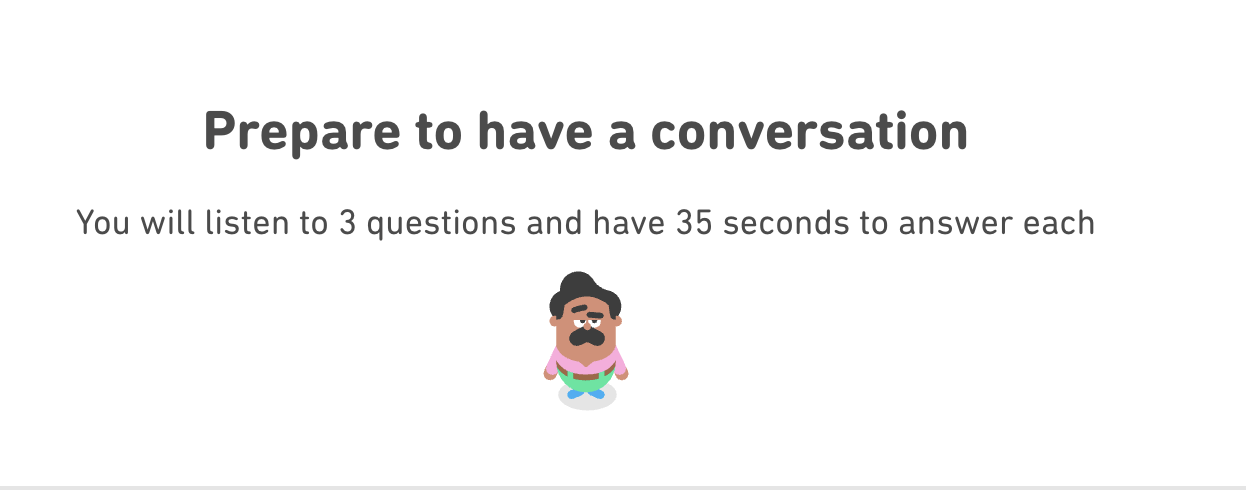
\includegraphics[width=\textwidth]{Fig5a.png}
% \label{fig5a}
% \end{minipage}%
% \qquad
% \begin{minipage}{0.43\textwidth}
% 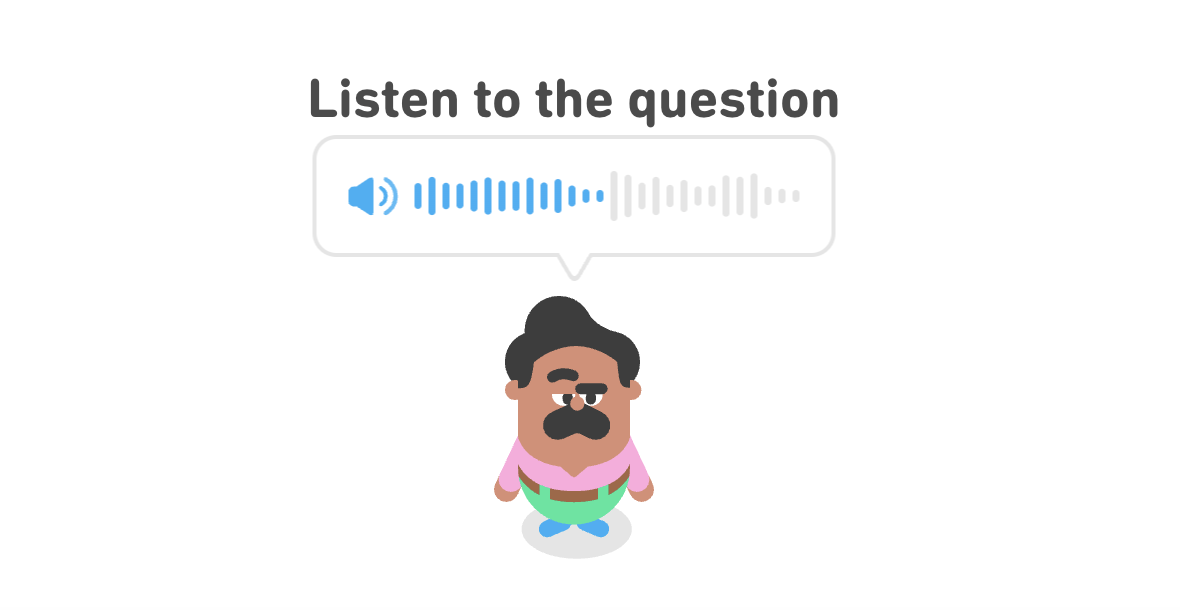
\includegraphics[width=\textwidth]{Fig5b.png}
% \label{fig5b}
% \end{minipage}%
%\end{figure}

%\begin{figure}[htbp]
% \centering
% \begin{minipage}{.5\textwidth}
% 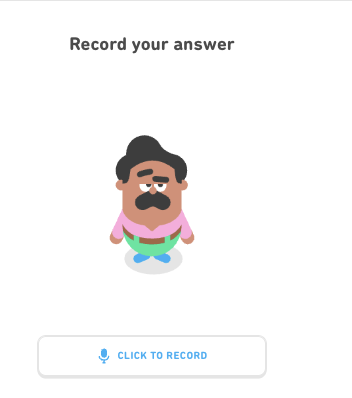
\includegraphics[width=\textwidth]{Fig5c.png}
% \label{fig5c}
% \end{minipage}%
% \qquad
% \begin{minipage}{0.45\textwidth}
% 
\includegraphics[width=\textwidth]{Fig5d.png}
% \label{fig5d}
% \end{minipage}%
% \caption{Compilation of screenshots of the Interactive Speaking Task of DET.}
% \source{\cite{duolingo2025format,duolingo2025practicehub}.} 
%\end{figure}

\begin{figure}[htbp]
    \centering
    % Primeira subfigura (a)
    \begin{subfigure}[a]{0.5\textwidth}
        \centering
        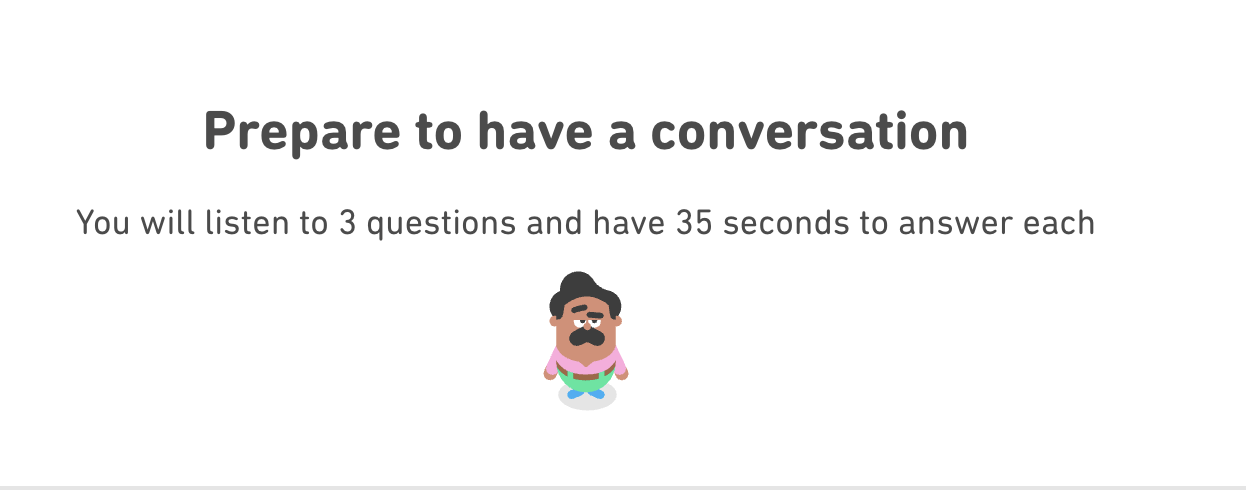
\includegraphics[width=\textwidth]{Fig5a.png}
        \label{fig5a}
    \end{subfigure}
    % Segunda subfigura (b)
    \begin{subfigure}[b]{0.4\textwidth}
        \centering
        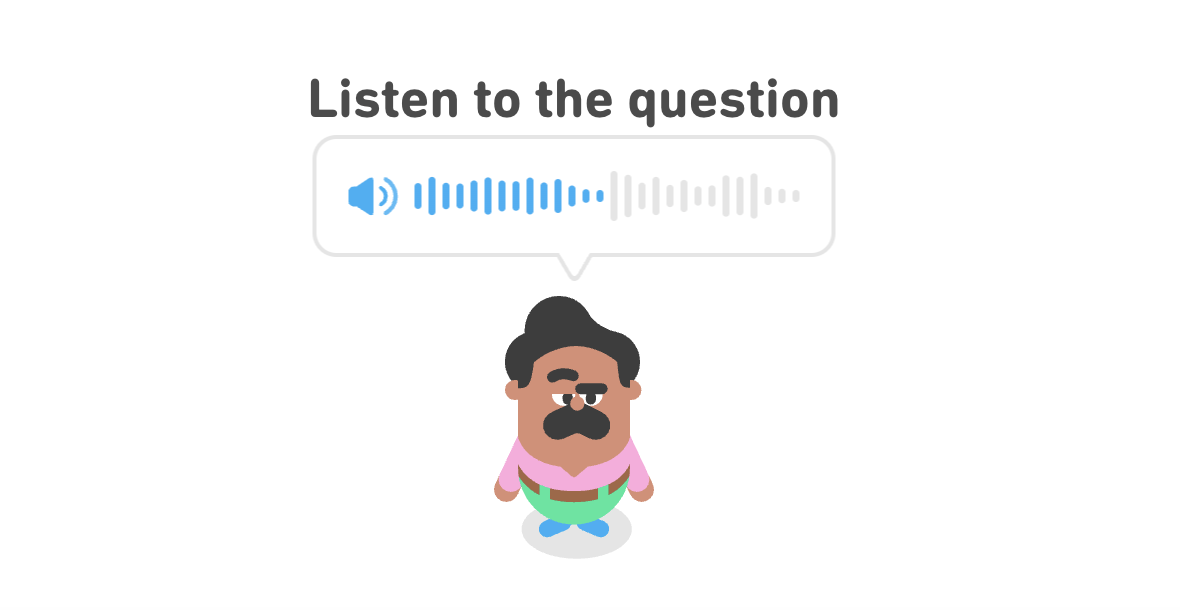
\includegraphics[width=\textwidth]{Fig5b.png}
        \label{fig5b}
    \end{subfigure}
     \begin{subfigure}[c]{0.3\textwidth}
        \centering
        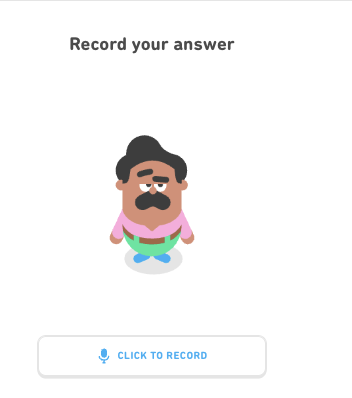
\includegraphics[width=\textwidth]{Fig5c.png}
        \label{fig5c}
    \end{subfigure}
     \begin{subfigure}[d]{0.3\textwidth}
        \centering
        
\includegraphics[width=\textwidth]{Fig5d.png}
        \label{fig5d}
    \end{subfigure}
    % Legenda geral da figura principal
    \caption{Compilation of screenshots of the Interactive Speaking Task of DET (a, b, c and d).}
    \source{\cite{duolingo2025format,duolingo2025practicehub}.} 
    \label{fig5}
\end{figure}

%Colocar letras a,b,c,d nas imagens?

Across the different iterations of the test, fictional, human cartoon-figured characters, such as a professor (\Cref{fig5}, a, b and c) and a student (\Cref{fig5}, d), facilitate the interaction with the user, acting as a proxy for the conventional examiner, as shown above. Unlike Lily, these are not conversational partners, but avatar interlocutors, indexing a university setting \cite{park2025assessing}. Thus, these characters visually reinforce the formality of the exam and the institutional authority that this test serves and is accountable to, as also evidenced by other markers in the text, such as formal language, time restrictions, etc. However, the cartoon style of the characters, with their low realism (low modality), mitigates the potentially daunting effect of the institutional power experienced by the user.

\begin{enumerate}[label=\alph*.]

    \item \textit{The opening screen (preparation)}
The opening screen of the Interactive Speaking component, as well as all the chosen screenshots here, is a multimodal text comprising image, writing, moving image and colour. The screenshot is framed by the title ‘Prepare to have a conversation’ followed by detailed instructions about the logistics of the exam, and is illustrated by the character of the professor, whose blinking eyes give the impression of a lively animation.

The directionality of gaze points towards the ‘Continue’ button below and works as a prompt. The mode of speech is suspended in this instance. The user is addressed in writing in the second person with the imperative ‘prepare’, along with the pronoun ‘you’ complemented by the gaze of the professor demanding attention.

As discussed above, the agency of the designers in this component is strictly regulating the flow of this conversation, with the AI – materialised in the vicarious animated figures – exercising very limited devolved agency in terms of the choice of characters and questions from a given repertoire aligned with exam-level requirements. With regard to the question of ‘who is speaking to whom’ in these screenshots, there seems to be some ambiguity for the users as to whether it is the fictional interlocutor, namely the professor figure, or the designers of the test. The users exercise their agency by reading through the screen and clicking on the ‘Continue’ button to proceed to the exam. However, this button is automatically activated after a few seconds, constraining the user’s agency.

    \item \textit{The setting of an aurally delivered task (listening)}

Two instructions are multimodally realised in this screenshot through the modes of writing and speech. The first instruction features as a title to the section, ‘Listen to the question’, whereas a second one emerges in speech as soon as this screen appears. Speech as a mode is complemented by the image of a soundwave within a rectangle and the icon of a loudspeaker activated throughout the spoken utterance. The figure of the professor is animated as his mouth, eyes and eyebrows move, and his head shifts in orchestration with speech, as a marker of the performed conversation of AI.

The effect of the imperative in the instruction featuring at the top of the screen – evocative of the authority of a classroom or exam setting – is mitigated by linguistic features in speech, such as the conditional “I would like…”. The interpersonal relationship is maintained through the ancillary role of the directionality of gaze and the facial expression with eyebrows moving.

The synergy of multimodal resources, including the tone of the voice, encourages the users while signposting the sequence and structure of the conversation: “\textit{I would like to ask you a few questions about…}”. In subsequent iterations of this interface, we see utterances such as: “\textit{I see, I have another question…}”, “\textit{Interesting…}” and “\textit{Thanks, let me ask you another question…}”.

The signposting offered by the character as simulated backchannelling forms a cohesive device and thus supports the enactment of a conversation with turn-taking. However, as there is no uptake by the character of any content that the user provides, there is only simulated coherence, as expected from a high-stakes test. The signposting is a marker of the restricted devolved agency of the AI, which chooses from a limited repertoire of responses. The design affords the user only a little time to think about their response, given that the transition to the next screen happens automatically.    

\item \textit{The delivery of the users’ response (speaking and recording)}

In this screenshot (\Cref{fig5} c), the title ‘Record your answer’ instructs the user to respond to the question, while a green button ‘Click to Record’ provides the entry to this recording. Subsequently, a ‘Submit audio’ button emerges on the screen, whereas a ‘Continue’ button appearing later activates the transition to the next question. While the user talks, a digital audio waveform visualising sound frequency with vertical bars appears as a marker of recording in progress, evidencing to the user that their recording is captured.

As the recording unfolds, the figure keeps changing his facial expressions, with eyes blinking, eyebrows waggling, mouth moving and gaze shifting, along with slight shifts of the head to the right and downwards. The constantly raised eyebrow potentially marks a sign of sustained interest and acknowledgement of the effort of the test taker. Despite the professor’s seriousness, his exaggerated facial expressions index humour and mitigate the effect of this potentially stressful high-stakes situation of the exam. Interestingly, when the users are instructed to press the ‘Submit’ and later the ‘Continue’ buttons, the professor character’s gaze and head point in that direction, visually reinforcing the instructions. It is worth noting that the facial expression of nodding is not included in the repertoire, as it could potentially be mistaken for an endorsement or value judgement of the answer.

The multimodality of the animation and, more specifically, the viewpoint and distance of the figure create a relaxed interpersonal relationship with the user. The professor is positioned lower than the user’s eye level, and despite the frontality of his face, his body is depicted as viewed from above, thus removing a marker of power. The animation simulates the engagement of an interlocutor, showing embodied interest and presence, while holding the space for the user to speak. The performance of the AI here forms an instance of simulated backchanneling, offering encouragement and acknowledgement to the user, signalling that the professor is attentive to their utterances. This is a visual marker of the designers’ intention to offer recognition of the user’s semiotic work, delivered through the performative agency of the AI.

The design features cater for the agency of the users as they click on the various buttons. Interestingly, the design does not allow the users to activate the ‘Submit’ button immediately; a sign of regulating their agency. This constraint is an implicit prompt to help them continue towards articulating a complete response.

Across all three screenshots (\Cref{fig5} a, b and c), it is evident that the agency of the designers is predominant – despite the occasional ambiguity as to whether it is the designers or the AI and the character talking to the user. The designers regulate and prompt the limited devolved agency of the AI, while facilitating the agency of the users in a systematic way (e.g., through written and oral instructions about topic, length of response and prompts for practical actions).

\end{enumerate}

\section{Discussion and conclusion}\label{sec-organizacao-latex}
In this study we analysed screenshots from different Duolingo designs for language learning and assessment and used them to make sense of the role and potential agency of AI in the realisation of these designs. Through a detailed MMSS analysis, we studied the materialities of these designs to attend to how human designers and the AI create the conditions for the user’s agency to be enacted. Overall, this study attends to how AI operationalises the Duolingo designers’ agency as an instance of compliance with institutional dictates in the broader sense, given that formal language education is largely institutionally regulated.

Each screenshot studied made simultaneously available the designs of three agents, the human designers, the AI and the user, bringing their contributions into one temporarily coherent and cohesive design. The analysis made it possible to identify the effect of the semiotic resources coming together and attribute them to the agency of the different parties involved, acknowledging that it is the agency of the user that makes it possible for this design to unfold as a text-in-action. The analysis has also substantiated the claim about the devolved, delegated and performed agency of AI as a proxy for the human designers’ agency. The latter is dominant in these learning designs and resonant with the regulatory frameworks within the world of education and language learning.

Across the different designs (the ‘Video Call with Lily’, ‘Role Play’, ‘Explain My Answer’ and the DET), we see that AI agency operates within institutional framings of English language skills and has fundamental guardrails and controls. AI also exercises different degrees of agency, which, in combination with the agency of the designers, create overall two different sets of conditions for users to interact: one characterised by more options for conversation and the other strictly regulated, as befits a high-stakes test.

Researching the agency of parties involved in such educational AI-assisted designs, it emerges that the human designers and their agency are dominant. Designers exercise their agency as language experts and policy experts with regard to: a) the standards against which language teaching should be measured, b) the level of difficulty in the tasks, and c) how progress can be accounted for. AI enacts and performs limited agency through delegation by human designers, who are the ones accountable to institutional standards.

In the institutionally regulated examples we have studied, there seems to be a syllabus and a distanced set of criteria and pedagogic principles as a point of reference in the development of AI-assisted designs. The designers have made an epistemological commitment \cite{bezemer2016multimodality} through deciding what English language knowledge to mediate, how it should be taught and why. AI also ‘converses’ with these institutional standards and choices of the designer, albeit in a devolved manner.

Different degrees of alignment with institutional discourses are evident in the various designs, as seen materialised through the analysis and corroborated further by the relevant Duolingo research (e.g., \textcite{burstein2022theoretical,park2025assessing}). In the ‘Video Call with Lily’, the character resonates with the informality of everyday conversation which the learning feature is supporting, with minimal accountability to authority. However, regulatory frameworks for levels of language proficiency, such as CEFR, still shape this design and are used as indicators of the user’s progress. CEFR is the metric against which the competence of the user is assessed informally by AI, forming the basis for AI to support the progression of the user through levels. In the Interactive Speaking component of the DET, the authority of the AI prompt offered is mitigated by the visuals linked to a cartoon genre. Nonetheless, as a high-stakes test linked to university admissions, the regulatory frameworks are heightened and more clearly visible to the user. For example, the DET test is regulated by four different frameworks \cite{burstein2022theoretical}.

The Duolingo designs brought together in this article realise a strong interpersonal relationship with the user through different multimodal resources, regulated differently in alignment with the purpose of the communication each one serves. These relationships are simulated and performed by the AI and realised differently across the examples, due to affordances in the design. However, the agency and voices of the human designers are constantly implicit, albeit mostly hidden behind the chatbot or characters enacting the devolved agency of the AI.

In the ‘Video Call with Lily’ and the ‘Role Play’, the computer adaptive technology facilitates an oral and a written conversation, respectively, enhanced by the multimodal features discussed above. The interaction between the user and the AI is designed to adjust to the user’s competency level on the basis of their contributions. Additionally, AI initiates an interpersonal relation through prompts, such as Lily’s comment “that’s interesting”, simulating a value judgement and an acknowledgement that a satisfactory response has been received.

In DET, an impression of conversation is given by the utterances of AI following on from the user’s responses, offering further signposting (e.g., "let us talk more about education") and re-prompting the user. This is reminiscent of what a human interviewer would have done in an exam context. These instances of simulated conversations often feature partial coherence and cohesion with the user’s utterances. Hence, we claim that AI performs and simulates agency in a manner evocative of a dialogic encounter (e.g., \textcite{duquepereira2025chatbots,tang2025dialogic}). However, as emphasised by \textcite[p. 3]{zappavigna2025emoji}, although the human-like conversational style of AI advances an illusion of genuine dialogue, it “remains purely computational, driven by extensive training datasets and complex algorithms”.

With the integration of AI in language learning designs, two questions arise: first, who are the agents involved in various instances in the making of the overall design as it unfolds in time, and second, how are these agents visible to the user and between which parties is the interpersonal relationship created? In the Duolingo examples, it emerges that the user encounters the interplay of multiple human agencies and the AI’s devolved agency, although not all of them are fully visible to the user. In interaction with these AI-assisted designs, the user navigates the conversation without necessarily being able to discern whether a feature is pre-designed by the human designers as a standard or generated by the AI as a response to their own prompts. However, the user can interact without needing to recognise the agents. As far as the user is concerned, the characters are proxies for both the AI and the human designers.

In our claim about performed and simulated agency for AI, we are largely aligned with \posscite{tomalin2025multimodal} work. This articulates the limitations of MMSS with regard to assigning agency to AI and offers a solution through his reframing of the theory. However, we think that the issue of whether AI sign-making equates to designing or not requires further research and context-specific elaborations, as it may not be pertinent to the case of the tightly regulated AI-assisted learning designs discussed here, but potentially be more apt for Gen-AI interactions.

In relation to the context studied here, we argue that sign-making (semiosis) cannot be teased apart from design, as they point to two facets of the same semiotic work of human agents. AI does generate text, but potentially a different term is needed to account for its role in communication. The position of \textcite{cope2024a_multimodal} – that meaning is more than text and that it cannot be separated from context – pertinently supports our argument above. Having access to context would require immersion into the social world as a social agent. AI cannot make value judgements and is not conditioned by socially shaped discourses (although it can be programmed to adopt ideological perspectives). Thus, it cannot position itself critically in relation to power or assess the context and the political and social dimensions of education directly and autonomously \cite{cope2024b_cybersocial}. Only human agency can be shaped by the social world and its discourses, arising as an endorsement or defiance of these discourses \cite{diamantopoulou2024agency}.

Following from this, we see a need to explore ways to make more visible the provenance and epistemological anchoring of sources of knowledge that AI draws on and transforms, as a way of responding to \posscite[p.~6]{cope2024a_multimodal} claim that AI “buries epistemic provenance”. Our claim about AI performing agency and being a proxy for human agency might be substantiated more systematically if we could trace the full process of engineering and inputs to AI (e.g., prompts, instructions, contexts) and repertoires and boundaries that human engineers have created.

A further implication of the above is the need to make more visible the limitations and potential of MMSS theory to account for the role of AI in the constantly changing communication landscapes, with shifts in the roles of designers and users and increasing refinement of AI (e.g., agentic AI). This would involve exploring whether new tools are needed for MMSS, and whether and how MMSS can be part of interdisciplinary approaches to designing or learning. This would require developing coherent and solid epistemological and ontological foundations for future research.

We also see the need for further research on the interaction between the stakeholders designing with AI and AI itself. Attending further to the dialogue between human designers and AI at the design stage will help us understand “the dynamic socio-technological interplays at work” \cite[p. 3626]{karimova2025dialogic}. This would also involve making more visible the many facets and nuances of the cyber-social relations between humans and AI \cite{karatza2024multimodal} and the way they are materialised in designs, further foregrounding the user perspective.

This study looked at AI-assisted language learning designs using MMSS as a theory of communication and learning \cite{bezemer2016multimodality}, anchoring all semiotic work onto the social. It endeavours to contribute to the discussion about the agency of AI in learning contexts, differentiating AI agency from the human agency required for sign-making and designing. AI-assisted designs for learning are always expected to have a social effect on the user, despite the fact that AI’s partial agentive participation in these designs does not originate in the social. AI can facilitate interaction, enabling learning. However, within the socially and politically shaped realm of education, there is an expectation that the human agents will be dominant to ensure alignment and control. For now, the agency of AI remains devolved, and should remain so, while humans retain the responsibility of critically shaping learning designs.


\printbibliography\label{sec-bib}
% if the text is not in Portuguese, it might be necessary to use the code below instead to print the correct ABNT abbreviations [s.n.], [s.l.]
%\begin{portuguese}
%\printbibliography[title={Bibliography}]
%\end{portuguese}


%full list: conceptualization,datacuration,formalanalysis,funding,investigation,methodology,projadm,resources,software,supervision,validation,visualization,writing,review
\begin{contributors}[sec-contributors]
\authorcontribution{Sophia Diamantopoulou}[conceptualization,datacuration,formalanalysis,investigation,methodology,validation,visualization,writing,review]
\authorcontribution{Sigrid Ørevik}[datacuration,formalanalysis,investigation,methodology,validation,visualization,writing,review]
\end{contributors}

\section*{\fontsize{10}{12}\selectfont Acknowledgements}
With special thanks to Dr Alina von Davier, Chief of Assessment at Duolingo, for her contribution to the conference paper \cite{vondavier2025designing} that has formed a starting point for this study, and for the permission to use the publicly available Duolingo materials included in the article. We would also like to thank both Dr Alina von Davier and Dr Xiangying Jiang from Duolingo for valuable clarifications on the examples used.

\section*{\fontsize{10}{12}\selectfont Use of AI}
We have used AI for generating literature and identifying readings and areas of scholarly work that relate to explorations of agency in AI related publications.

\begin{dataavailability}
\txtdataavailability{nodata} % options: dataavailable, dataonly, databody, datanotav, nodata
\end{dataavailability}




\end{document}

